\documentclass{hertieteaching}
\addbibresource{/Users/wlowe/Bibliography/zotero.bib}

\usepackage{relsize}

\title{Scaling}

\begin{document}

{\setbeamertemplate{footline}{}
\begin{frame}
\maketitle
\end{frame}}
\addtocounter{page}{-1}

%%%
\begin{frame}{Scaling}

We can think about document living in some kind of \textit{space} with $\theta$ as the positione.g.
\begin{itemize}
  \item affect, a.k.a. \textit{sentiment analysis}
  \item unidimensional policy preferences
  \item multidimensional ideological position
\end{itemize}

How to place documents in space?
\begin{itemize}
  \item Think of a row in the document term matrix as a vocabulary profile, e.g. by normalize the counts
  \item This is a point in a (very high-dimensional) space
  \item Which has distances to every other document in that space
\end{itemize}
But we can also collapse them down into a smaller space, e.g. one or two dimensions
\begin{itemize}
  \item Often we think they really live there
  \item Sometimes it's just visualization
\end{itemize}
\end{frame}

\begin{frame}{Plan}
\begin{itemize}
  \item Where does information about position live?
  \item The model
  \item Spatial talking
  \item Special cases
  \item Validation
  \item Comparing positions
\end{itemize}


\end{frame}


\begin{frame}{Reminder}

A matrix of document by word/topic counts is a \textit{contingency table}

\begin{center}{\scriptsize
\begin{tabular}{rrrrrrrr} \toprule
          & neue & vor &Menschen& wie &nur & Arbeitsplätze & \ldots \\ \midrule
...\\
FDP-2005  &    11 & 20  &      6 & 22  &31 &            17 & \ldots\\
FDP-2002  &    17 & 17  &     27 & 30  &35  &            9 & \ldots\\
PDS-2005  &     5 & 10  &     17 & 10  & 9   &          12& \ldots\\
PDS-2002  &    15 & 19  &      8  & 9  & 3    &          9& \ldots\\
GREENS-2005  & 42 & 21    &   47 & 46 & 19 &            17& \ldots\\
GREENS-2002  & 27 & 18    &   27 & 28  &22 &            21& \ldots\\
SPD-2005  &     8 & 15 &      26 & 11 & 13     &        10& \ldots\\
SPD-2002  &    16 & 18 &      16 & 16 &  9      &        7& \ldots\\
CDU-2005  &    21 & 12 &      10 & 13 & 19       &      22& \ldots\\
CDU-2002  &    20 & 20 &      14 & 15 & 18        &      7& \ldots\\ 
...\\
\bottomrule
\end{tabular}}
\end{center}

\end{frame}

\begin{frame}{Scaling: Party position dynamics}

\centerline{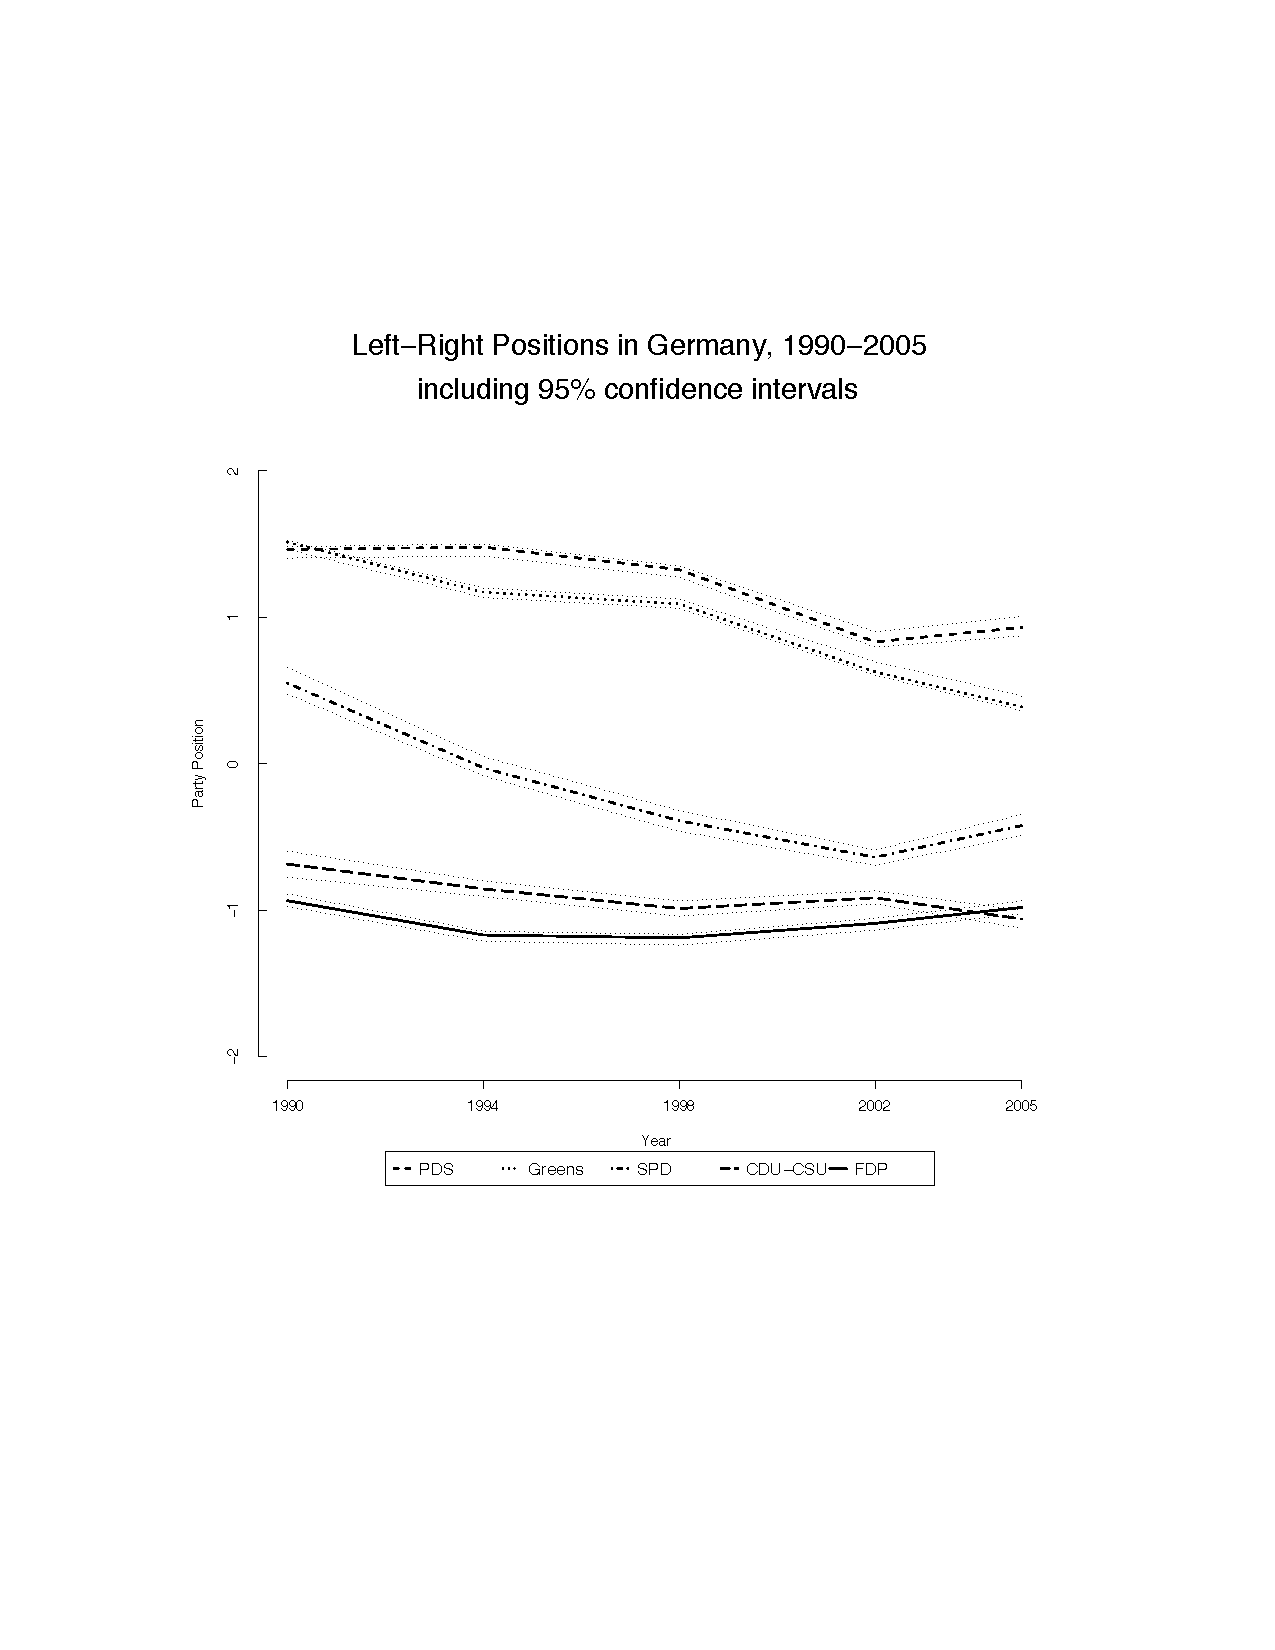
\includegraphics[scale=0.4]{pictures/poissonscaling}}
German party position on the economy \parencite{Slapin.Proksch2008}

\end{frame}


\begin{frame}{Scaling: Irish budget debates}

\centerline{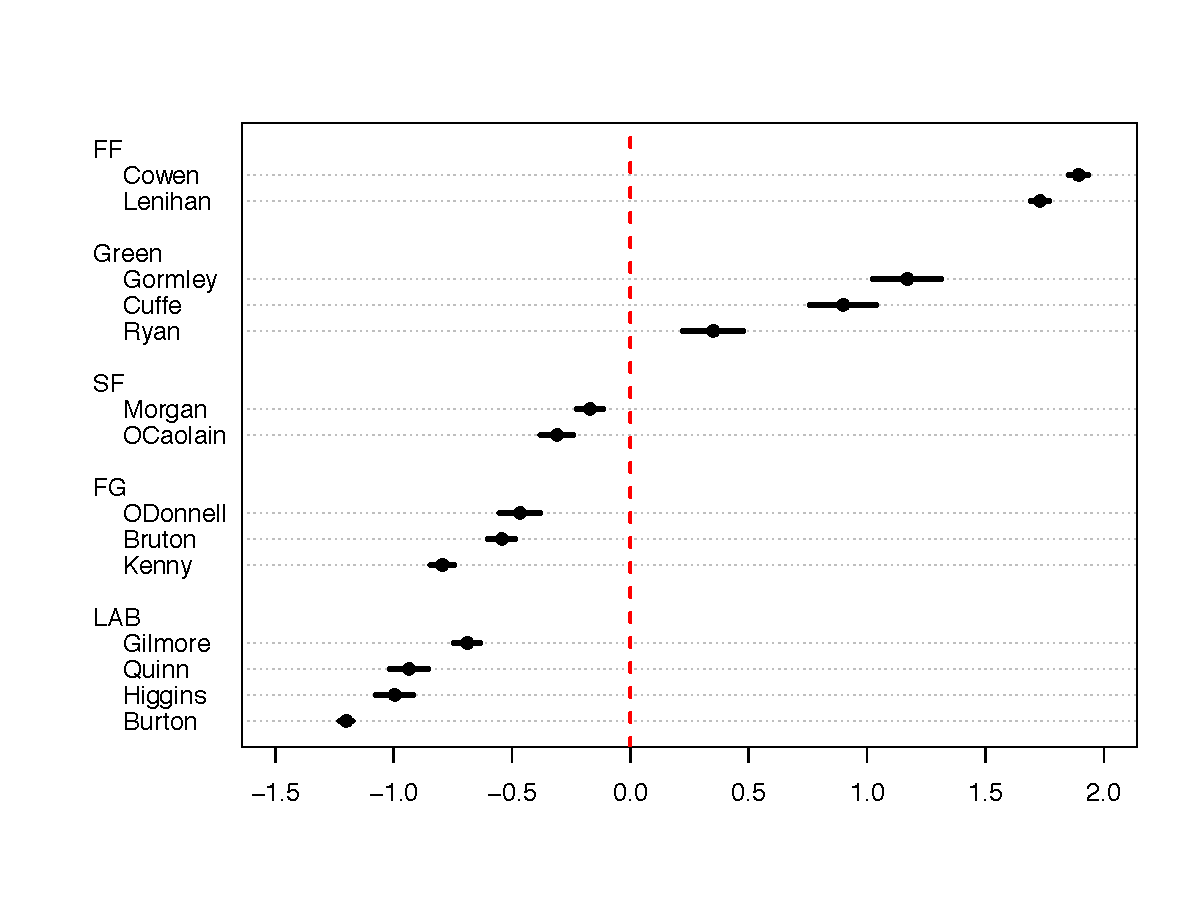
\includegraphics[scale=0.45]{pictures/dotplot_hscaled}}
Estimated FOMC member ideal points from meeting transcripts  \parencite{Lowe.Benoit2013}

\end{frame}

\begin{frame}{Scaling: fomc transcripts}

\centerline{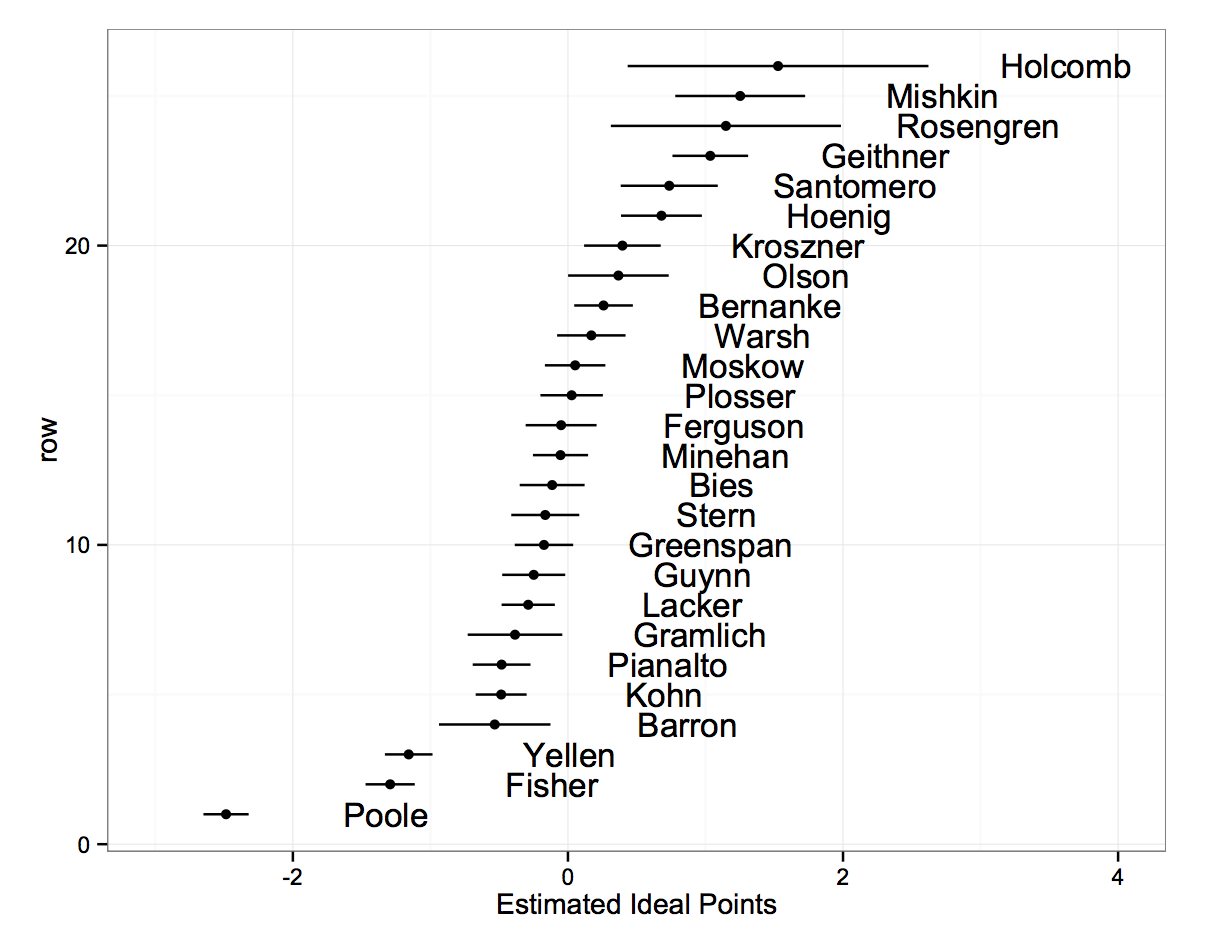
\includegraphics[scale=0.35]{pictures/fomc-ip}}
Estimated FOMC member ideal points from meeting transcripts  \parencite{Baerg.Lowe2020}

\end{frame}

\begin{frame}{Scaling: Senators (Monroe \& Maeda)}

\centerline{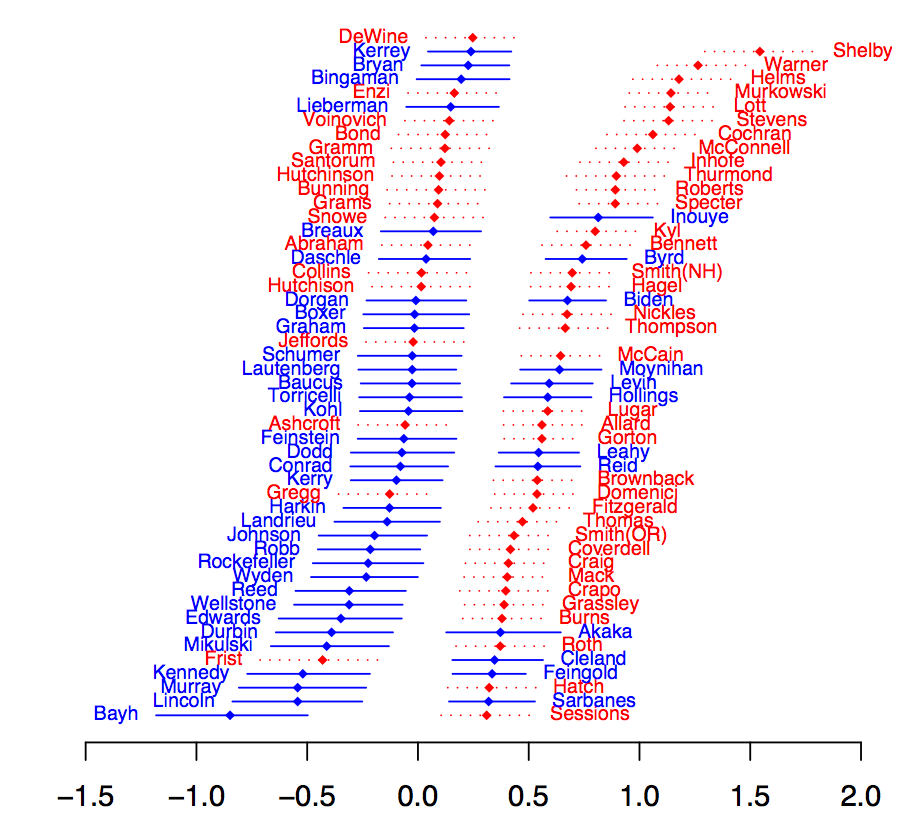
\includegraphics[scale=0.25]{pictures/senator-ip-monroe-maeda} }
Samizdat from \parencite{Monroe.Maeda2004}

\end{frame}


\begin{frame}{Where positional information lives}

\begin{center}{\scriptsize
\begin{tabular}{lllrrrr}\toprule
      &            &        Word \\ \midrule
      &     Party  &  Wirtschaft & soziale & Förderung & \ldots \\ \midrule
2002  &     FDP       &       14 &       4 &        15 & \\
      &     CDU       &       11 &       8 &        20 & \\
      &     SPD       &       15 &       9 &        10 & \\
      &     PDS       &        7 &      16 &         9 & \\
      &     Grüne     &        2 &      41 &        12 & \\
      &     \ldots \\ \bottomrule
\label{fragment}
\end{tabular}}\end{center}

Assumptions:
\begin{itemize}
  \item Position does not depend on \textit{document length}
  \item Position does not depend on \textit{word frequency}
\end{itemize}

\pause 

Implication
\begin{itemize}
  \item table margins are uninformative
\end{itemize}


\end{frame}
\begin{frame}{Where positional information lives}

\begin{center}{\footnotesize
\begin{tabular}{lllrrrr}\toprule
      &            &        Word \\ \midrule
      &     Party  &  Wirtschaft & soziale & Förderung & \ldots \\ \midrule
2002  &     FDP       &      {14} &      {4} &        15 & \\
      &     \textcolor{red}{CDU}       &      \textbf{11} &      \textbf{8} &        20 & \\
      &     SPD       &       15 &       9 &        10 & \\
      &     PDS       &        7 &      16 &         9 & \\
      &     Grüne     &        2 &      41 &        12 & \\
      &     \ldots \\ \bottomrule
\label{fragment}
\end{tabular}}\end{center}

That leaves only \textit{association structure}.

\pause

The CDU uses 'Wirtschaft' (business) 11/8 = 1.38 times more than 'soziale' (social).
\end{frame}

\begin{frame}{Where positional information lives}

\begin{center}{\footnotesize
\begin{tabular}{lllrrrr}\toprule
      &            &        Word \\ \midrule
      &     Party  &  Wirtschaft & soziale & Förderung & \ldots \\ \midrule
2002  &     \textcolor{red}{FDP} &      \textbf{14} &       \textbf{4} &        15 & \\
      &     CDU       &      {11} &      {8} &        20 & \\
      &     SPD       &       15 &       9 &        10 & \\
      &     PDS       &        7 &      16 &         9 & \\
      &     Grüne     &        2 &      41 &        12 & \\
      &     \ldots \\ \bottomrule
\label{fragment}
\end{tabular}}\end{center}

The FDP uses 'Wirtschaft' (business) 14/4 = 3.5 times more than `soziale' (social). 
\end{frame}

\begin{frame}{Where positional information lives}

Many $(N-1)(V-1)$ small but relevant facts about relative proportional emphasis
\begin{itemize}
\item[1.] FDP's emphasis on Wirtschaft over soziale is 3.5/1.375 = 2.55 times larger than that of the CDU.  
\item[2.] CDU's emphasis on Wirtschaft over soziale is 0.82...
\item[3.] \ldots
\end{itemize}

You might recognize 2.55 and 0.82 and so on as \textit{odds ratios}
\begin{align*}
\frac{P(\text{Wirtschaft} \mid \text{FDP})} 
     {P(\text{soziale} \mid \text{FDP})} \bigg/
\frac{P(\text{Wirtschaft} \mid \text{CDU})} 
     {P(\text{soziale} \mid \text{CDU})}     & = \frac{14}{4} \bigg/ \frac{11}{8} 
\end{align*}
which are delightfully indifferent to document lengths and word frequencies.\footnote{Add $k$ the frequency of Wirtschaft, keeping the odds ratio the same, and notice that it just adds (some function of) $k$ to both numerator and denominator, which cancel.}


\end{frame}
\begin{frame}{Where positional information lives}


Actually this is where \textit{all} substantively interesting information in document term matrices lives
\begin{itemize}
  \item where else is there?
\end{itemize}

Any kind of text model, e.g. a topic model
\begin{itemize}
  \item implies constraints on how these odds ratios can vary
  \item reduces the dimensionality of word distributions to a lower than $V$ space
\end{itemize}


\bigskip
So let's think about building a model of them from first principles

\end{frame}


\begin{frame}{Modeling the associations}
First we'll assume that each $C_\mathit{ij}$ is a Poisson distributed with some expected rate
\begin{align*}
C_\mathit{ij} & \sim \text{Poisson}(\mu_\mathit{ij}) 
\end{align*}

\pause 

There are two \textit{log-linear models} of any contingency table
\begin{align*}
\text{log}\, \mu_\mathit{ij}  & = \alpha_{i} + \psi_{j} & \text{({boring})}\\ 
              & = \alpha_i + \psi_{j} + \lambda_\mathit{ij} & \text{({pointless})}
\end{align*}

\end{frame}

\begin{frame}{Modeling the associations}
	
First we'll assume that each $C_\mathit{ij}$ is a Poisson distributed with some expected rate
\begin{align*}
C_\mathit{ij} & \sim \text{Poisson}(\mu_\mathit{ij}) 
\end{align*}

	
There are two \textit{log-linear models} of any contingency table
\begin{align*}
\text{log}\, \mu_\mathit{ij} & = \alpha_{i} + \psi_{j} & \text{(independence)}\\
              & = \alpha_i + \psi_{j} + {\color{HertieSchoolRed} \lambda_\mathit{ij}} & \text{(saturated)}
\end{align*}

\pause

All the \textit{relative emphasis}, all the odds ratio information, and all the \textit{position-taking} is in $\lambda$

Reminder: 
\begin{itemize}
  \item In log linear model land, the matrix of $\lambda$ values is just the same size as $C$
  \item but the influence of the row and column margins has been \textit{removed} by the $\alpha$ and $\psi$ parameters
\end{itemize}
 


\end{frame}





%%%%%%%%%%%%%%%%%%%%%%%%%%%%%%%%%%%%%%%%%%%%%%%%

\begin{frame}{Infer dimensional structure}

Intuition: $\lambda$ has an orthogonal decomposition
\begin{align*}
\lambda & = \Theta\Sigma B^T & \text{{\normalsize (SVD)}}\\
                  &= \sum^{M}_{m} \theta_{(m)} \sigma_{(m)} \beta_{(m)}^T\\
                  &\approx \textcolor{black}{\theta}\,\textcolor{black}{\sigma}\,\textcolor{black}{\beta}^T & \text{{\normalsize (Rank 1 approx.)}}
\end{align*}

\textcolor{black}{$\theta$} are \textit{document positions}

\textcolor{black}{$\beta$} are \textit{word positions}

\textcolor{black}{$\sigma$} says \textit{how much relative emphasizing} is happening in this dimension

\end{frame}

\begin{frame}{singular value decomposition}

\bigskip
\centerline{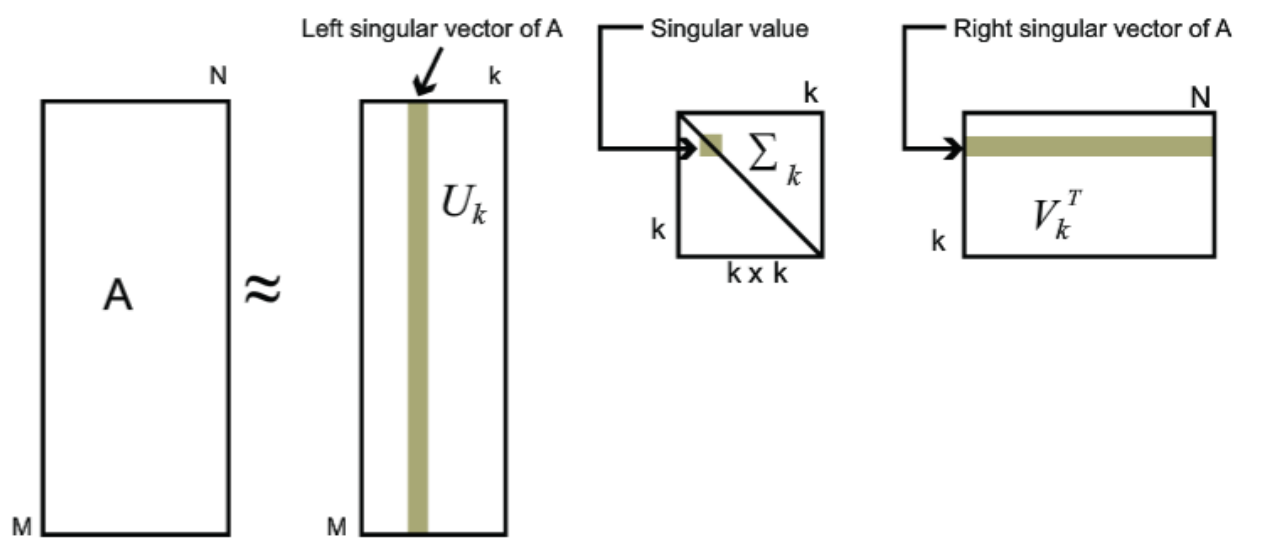
\includegraphics[scale=0.6]{pictures/svd}}

\medskip
where $A$ is our $\lambda$, $U$ is our $\theta$ and $V$ is our $\beta$
\end{frame}



\begin{frame}{Modeling proportional relative emphasis}

That small fact from earlier
\begin{itemize}
  \item FDP's emphasis on 'Wirtschaft' over 'soziale' is 3.5/1.375 = 2.55 
times larger than that of the CDU.
\end{itemize}

According to the model:
$$
\text{log}\left(\frac{3.5}{1.375}\right) ~\approx~ (\theta_\text{FDP} - \theta_\text{CDU}) ~\sigma~ (\beta_\text{Wirtschaft} - \beta_\text{soziale})
$$
\end{frame}
\begin{frame}{This is a very good idea}

Everybody has it...
\begin{itemize}
  \item Ecology, archaeology, psychology, political science
\end{itemize}
and has been having it since \textcite{Hirschfeld1935}, as
\begin{itemize}
  \item the RC Association model \parencite{Goodman1981}
  \item Wordfish \parencite{Slapin.Proksch2008}
  \item Rhetorical Ideal Points \parencite{Monroe.Maeda2004}
\end{itemize}

\bigskip
\pause

That was just algebra -- \textit{why} is this a very good idea?
\end{frame}

\begin{frame}{Spatial talking}

\begin{columns}[T,onlytextwidth]
\column{0.45\textwidth}
How much will each party use word $b$?
\bigskip

\centerline{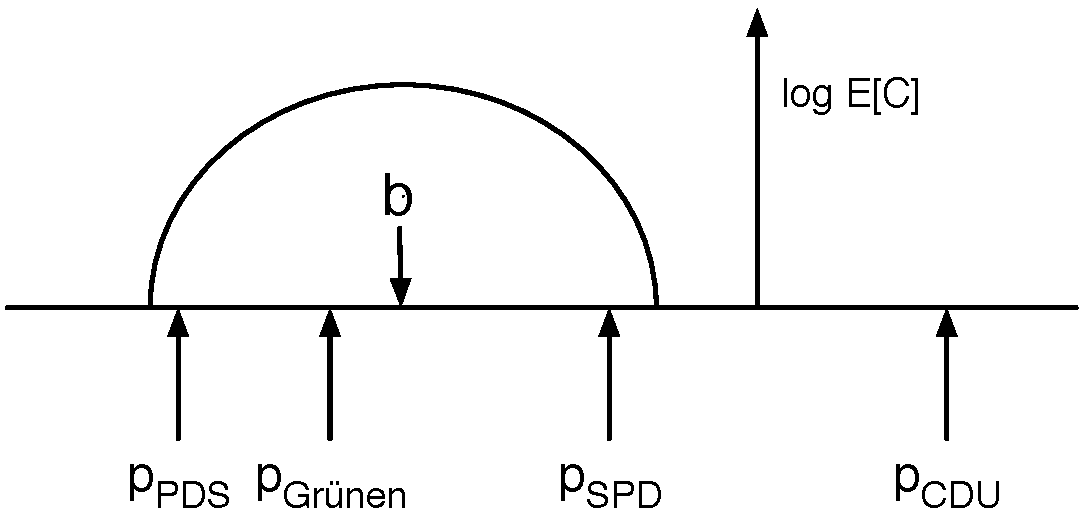
\includegraphics[scale=0.3]{pictures/ip-schematic2}}

\medskip
As a model
$$
\text{log}~\mu_\mathit{ij}~ = r_i + c_j ~+~ \frac{(p_i - b_j)^2}{v}
$$
where $v$ describes how fast the tendency to 
say $b$ declines with distance
\pause
\column{0.55\textwidth}
That we've seen before

\begin{align*}
r_i + c_j &+~\frac{(p_i - b_j)^2}{v}\\
r_i + c_j &+~ (p_i^2 - 2p_i b_j + b_j^2) / v\\
\underbrace{(r_i + p_i^2 / v)}_{\alpha_i} + 
  \underbrace{(c_j + b_j^2 / v)}_{\psi_j} &+ ~
  \underbrace{p_i}_{\theta_i} 
  \underbrace{(1/v)}_{\sigma}
  \underbrace{(-2 b_j)}_{\beta_j}
\end{align*}

For the microeconomists, think
\begin{itemize}
  \item stochastic utility decision model with $V$ choices
  \item and very simple underlying preference structure
  \item i.e. a huge structured IIA violation\ldots
\end{itemize}


\end{columns}


\end{frame}

\begin{frame}{For the political scientists}

\begin{columns}[T,onlytextwidth]
\column{0.5\textwidth}
\centerline{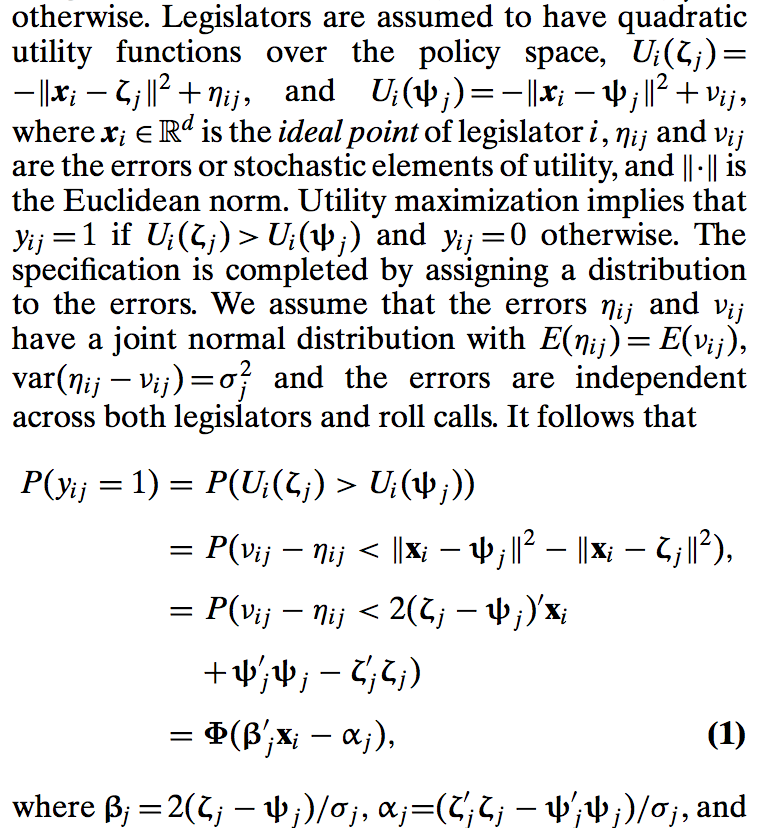
\includegraphics[scale=0.45]{pictures/ideal}}
\column{0.05\textwidth}
\column{0.45\textwidth}


$\longleftarrow$ from \textcite{Clinton.etal2004}
\medskip

Condition on document length to get a spatial `voting' model \parencite[via the `Multinomial-Poisson' transform',][] {Baker1994,Lang2004}

\end{columns}
	
\end{frame}


\begin{frame}{For the political scientists}

\centerline{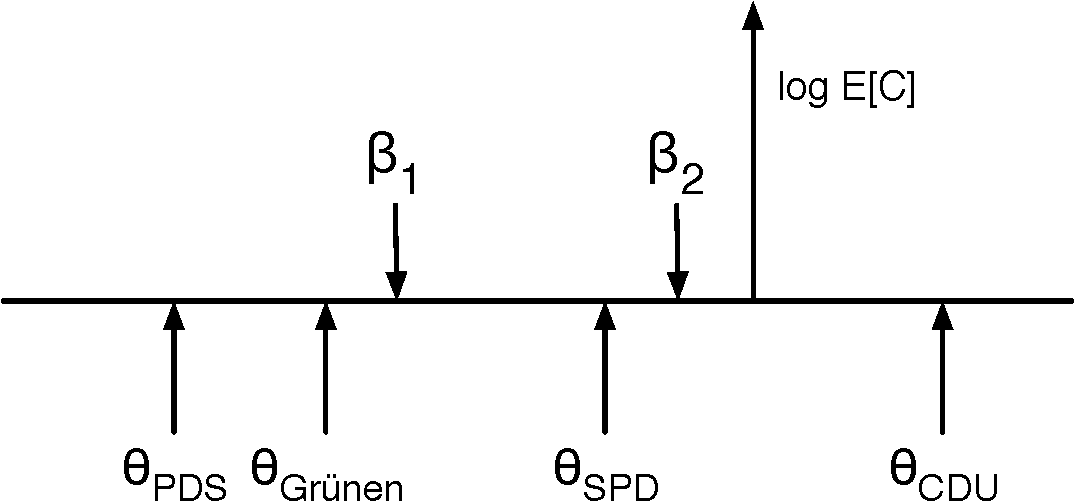
\includegraphics[scale=0.4]{pictures/ip-schematic3-cropped}}
\medskip

Decision time: Should I say word 1 or word 2?
\begin{itemize}
  \item Depends on my distance to each of them
  \item If I can say the word exactly once before being presented with another pair then this is the roll-call voting context and this is a logistic regression (embedded in an IRT model) 
\end{itemize}
\end{frame}


%Assume 2 word types with positions $\beta_1$ and $\beta_2$ and $N_i$ words

%Condition on document lengths to get an equivalent IRT model *(MP transform, e.g. Baker 1994, Lang 2004)*
%\begin{align*} 
%[C_{i1}\ldots C_{iJ}] &\sim \text{Multinomial}( {\pi}_{i1} \ldots \pi_{iJ},  N_{i} )\\
%\pi_{ij} &= \mu_{ij} / \sum^{J}_j \mu_{ij} \\
%\text{log}\!\bigg(\frac{\pi_{ij}}{\pi_{ik}}\bigg) &= \text{log}~ \pi_{ij} - \text{log}~ \pi_{ik}\\
% &= (\alpha_i - \alpha_i) + (\psi_j - \psi_k) + \theta_i\,(\beta_j - \beta_k)\\
% &= ~~~~~~~~~~~~~~~~~~~\;\;\;\;\;\,\psi_{j/k}~~\;\;\, + \textcolor{black}{\theta_i}\;~\;\;\;\textcolor{black}{\beta_{j/k}}
%\end{align*}


%\begin{frame}{Just like spatial voting}
%
%\centerline{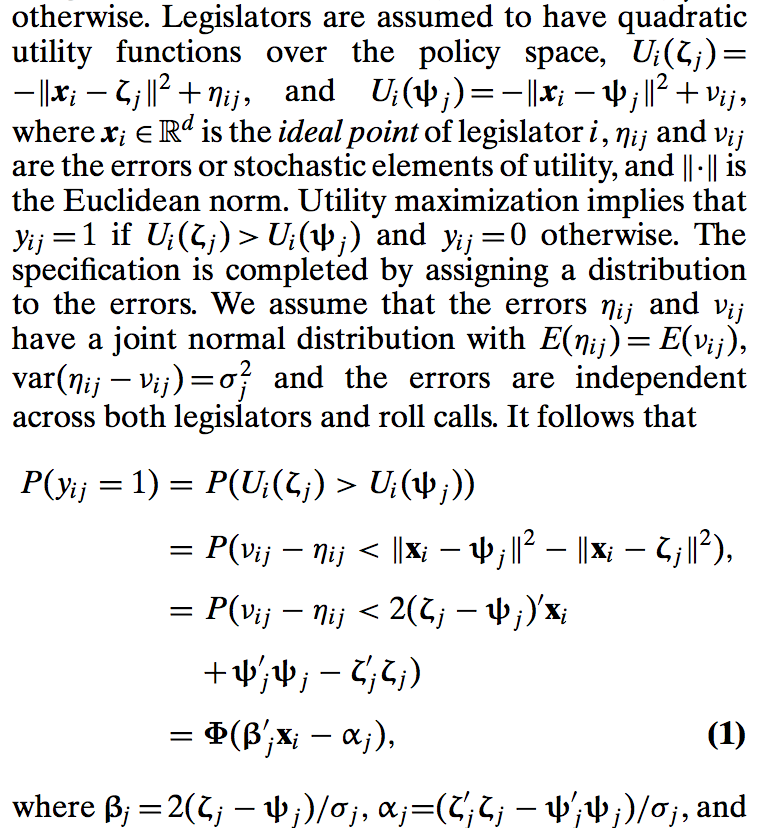
\includegraphics[scale=1]{pictures/ideal}}
%
%from \textcite{Clinton.etal2004a}
%
%\end{frame}
%\begin{frame}{Just like spatial voting}
%
%\centerline{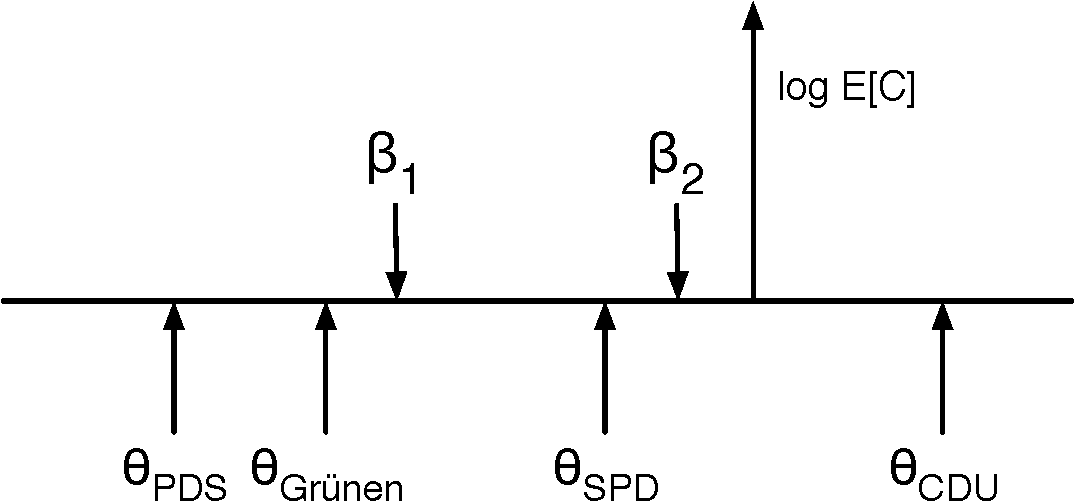
\includegraphics[scale=.4]{pictures/ip-schematic3-cropped}}
%
%
%
%\end{frame}
%\begin{frame}{Scaling with two words or topics}
%
%\begin{align*} 
%[C_{i1}, C_{i2}] &\sim \text{Binomial}( [{\pi}_{i1}, \pi_{i2}],  N_{i} )\\
%\pi_{i1} &= \mu_{i1} / (\mu_{i1} + \mu_{i2}) \\
%\text{log}\!\bigg(\frac{\pi_{i1}}{\pi_{i2}}\bigg) &= \text{log}~ \pi_{i1} - \text{log}~ \pi_{i2}\\
% &= (\alpha_i - \alpha_i) + (\psi_1 - \psi_2) + \textcolor{black}{\theta_i}\,(\textcolor{black}{\beta_1} - \textcolor{black}{\beta_2})\\
% &= ~~~~~~~~~~~~~~~~~~~\;\;\;\;\;\,\psi_{1/2}~~\;\;\, + \theta_i\;~\;\;\;\beta_{1/2}
%\end{align*}
%
%Quadratic utility generates a decision boundary log-linear in the 
%difference between word/topic positions.
%
%\end{frame}

\begin{frame}{Special cases: rile}

According to the folk at the WZB \parencite{Budge.etal1987,Volkens.etal2020}, parties signal their ideology by making just such a sequence of choices, over topics
\begin{itemize}
  \item Manually identify `Right' topics $R$ and `Left' topics $L$, from a 56 topic codebook
  \item For each party manifesto, sum up the Right topic proportions and subtract the sum of the Left topic proportions
  \item That's Right-Left position, a.k.a. \textit{RILE}
\end{itemize}
\begin{align*}
\hat{\theta}_i &=~ \mathlarger{\sum}_{j \in R} \frac{C_\mathit{ij}}{C_\mathit{i.}} -
                 \mathlarger{\sum}_{k \in L} \frac{C_\mathit{ik}}{C_\mathit{j.}}& &\text{RILE}\\
                 \intertext{where}
C_\mathit{i.} &=~ \sum_{j} C_\mathit{ij}                
\end{align*}
is the document length
%
%ideology 
%Identify left L and right R categories 
%
%
%and compute logits  
%\parencite{Lowe.etal2011}
%$$
%\hat{\theta}_i = \text{log}\,\,\, \frac{\sum_{j \in R}C_{ij}}{\sum_{k \in L}C_{ik}}
%$$
%$\hat{\theta}$s are linear in model $\textcolor{black}{\theta}$
%
%For our colleagues in psychophysics
%\begin{itemize}
%  \item Position is relative **proportional** emphasis (the Weber-Fechner law)
%\end{itemize}

\end{frame}
\begin{frame}{Consequences: Validation}

%This aggregation will presumably be valid for \textit{ideological similar} categories

Open questions:
\begin{itemize}
  \item Are these the correct category choices?
  \item How could we get policy-specific scales? \parencite{Lowe.etal2011,Benoit.etal2012a}
  \item What about new categories -- where do they fall, ideologically speaking?
\end{itemize}

Some intermediate answers \parencite{Lowe.etal2011}
\begin{itemize}
  \item Probably, but the functional form is not a difference of proportions
\begin{align*}
\hat{\theta}_i & = \text{log} \frac{\sum_{j \in R} C_{ij}}
                                   {\sum_{k \in L} C_{ik}} & & \text{logit scores}
\end{align*}
  \item By careful manual choice of categories
  \item ??
\end{itemize}

\end{frame}
\begin{frame}{Consequences: Validation}


Better answer: Let's check
\begin{itemize}
  \item We know already that logit scores are a special case of the model with two `words'
\end{itemize}


Plan:
\begin{itemize}
  \item Fit the scaling model -- here to post-1989 Germany
  \item See if the $\theta$s agree with \textit{RILE}
  \item See if the $\beta$s fall into two homogenously position groups
  \item Get scores for topics not in $L$ and $R$
\end{itemize}


\end{frame}

\begin{frame}{rile and other categories}

\centerline{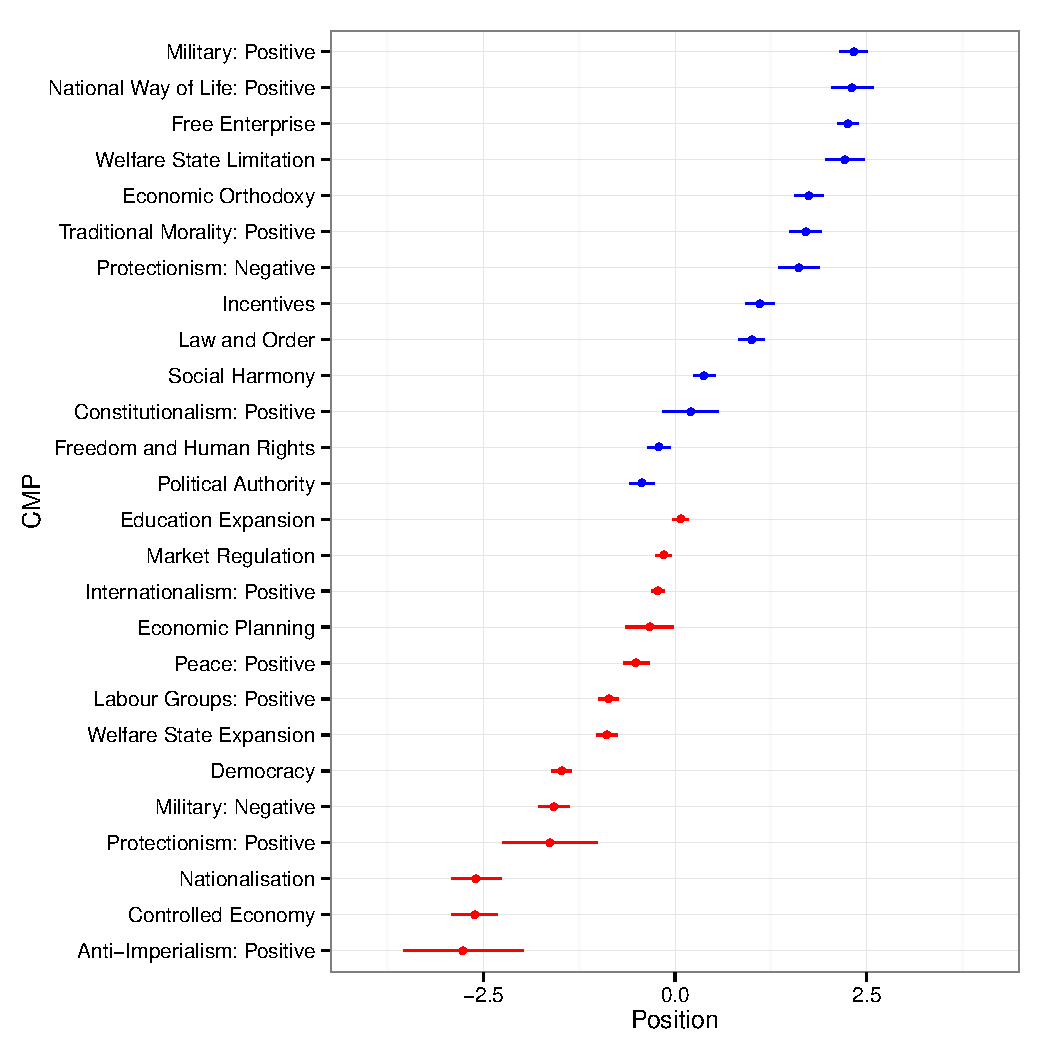
\includegraphics[scale=0.4]{pictures/rile-cats}\pause 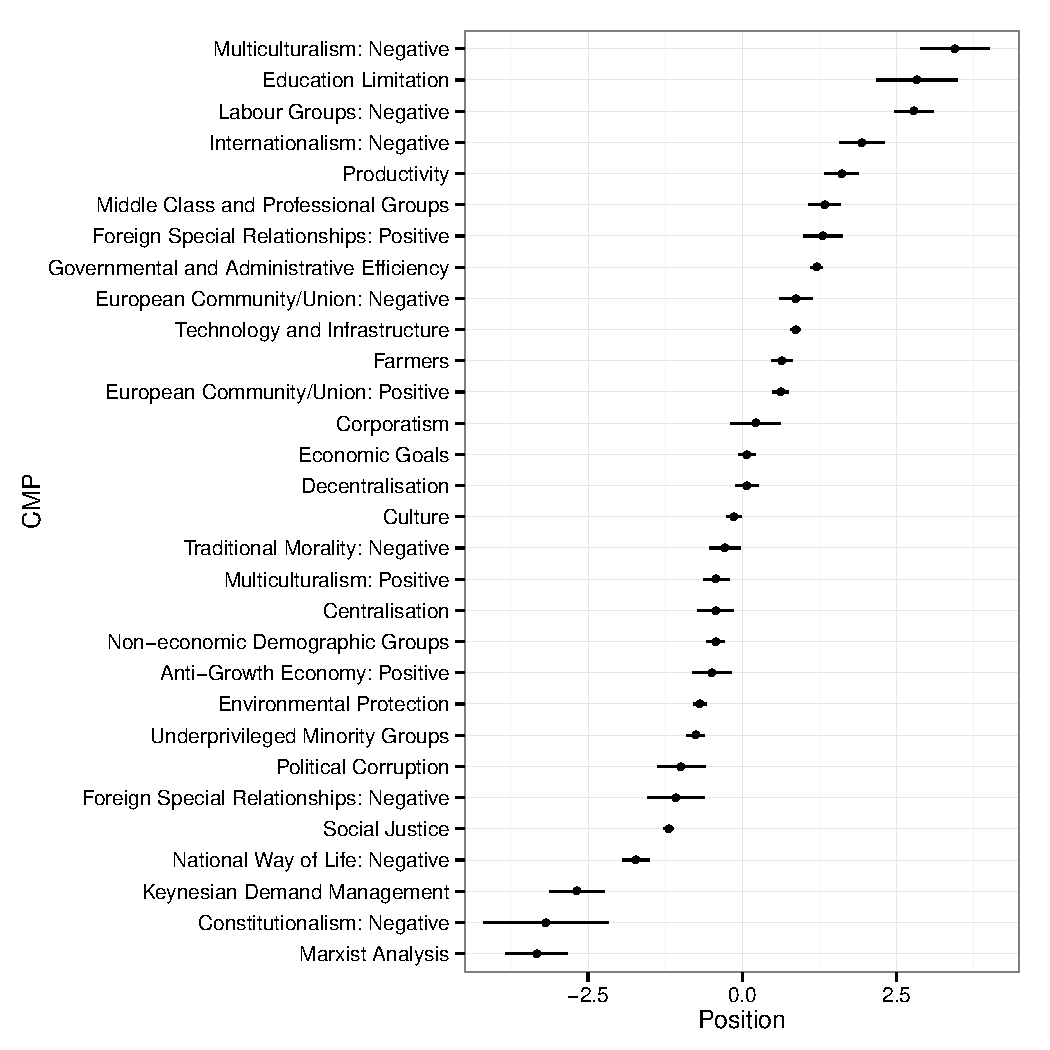
\includegraphics[scale=0.4]{pictures/non-rile-cats}}
\end{frame}

\begin{frame}{Brits\ldots}

\centerline{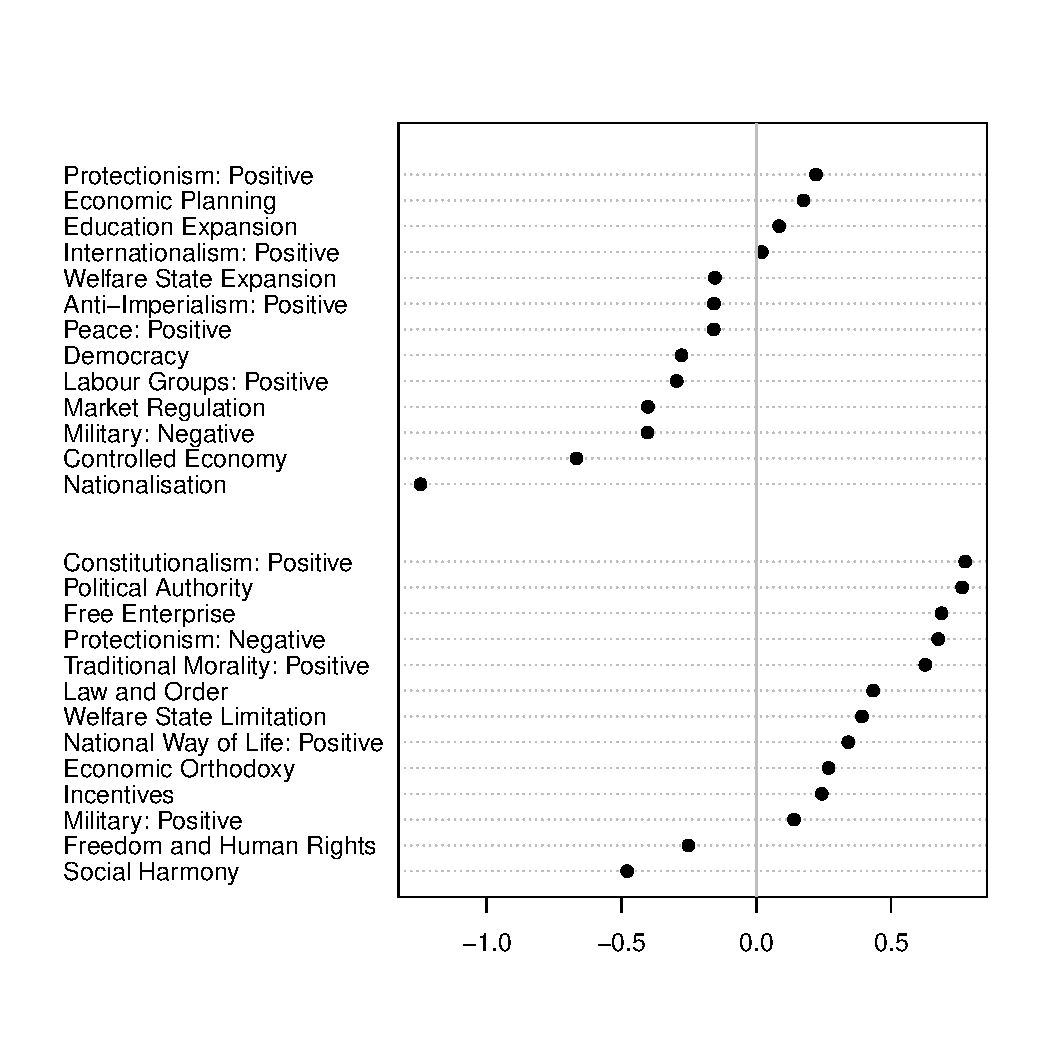
\includegraphics[scale=0.4]{pictures/UK_items}\pause 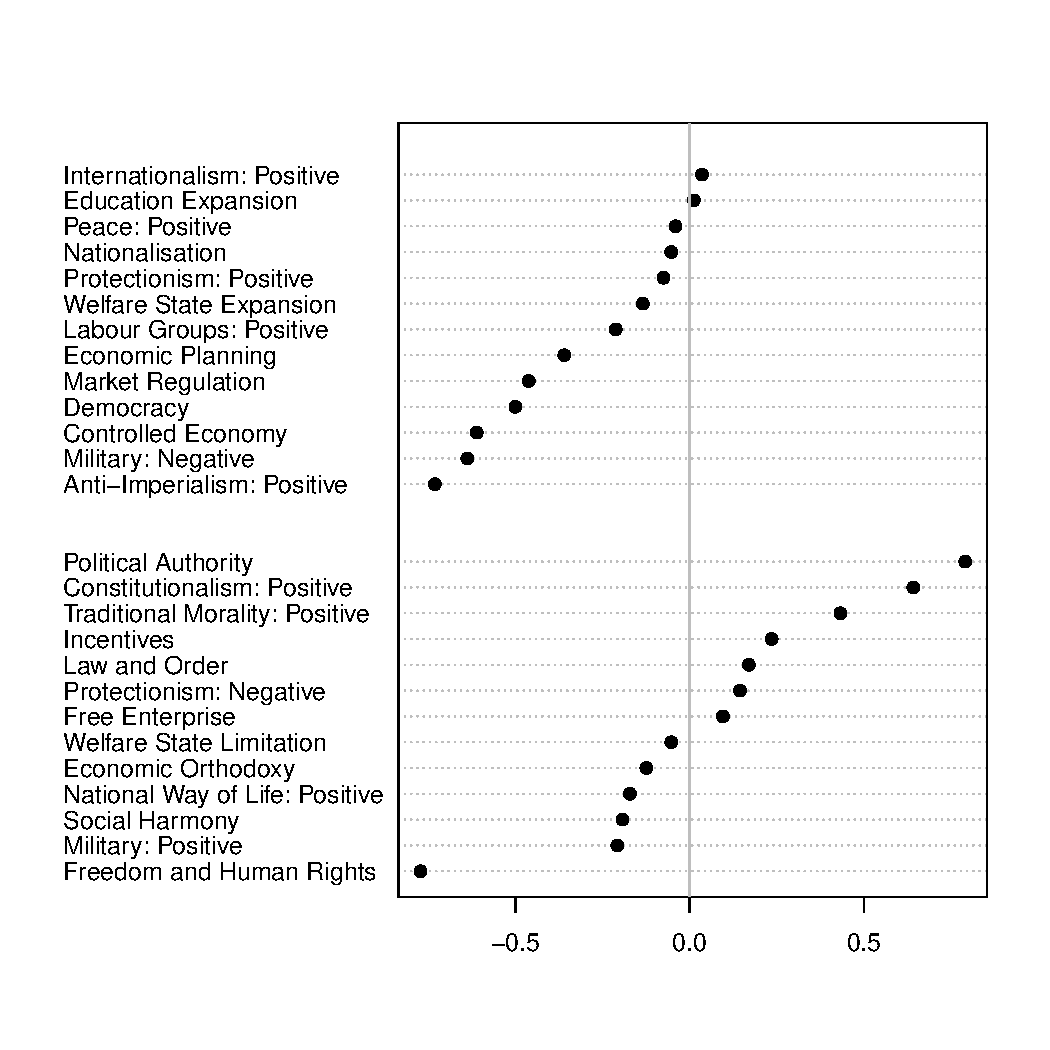
\includegraphics[scale=0.4]{pictures/UK_items_only_main_parties}}
\end{frame}

\begin{frame}{Theoretical questions}

\begin{itemize}
  \item How can we know what $\theta$ represents?
  \item How can we get policy-specific scores?
  \item How comparable are these document and word position estimates?
  \item (When) does it make sense to project different documents into a space
  \item What would a multi-dimensional version of this model look like
\end{itemize}

\end{frame}

\begin{frame}{Implementations}

\textsc{Association model}
\begin{itemize}
  \item What quanteda calls `wordfish'
  \item limited to scaling in one dimension
  \item Provides uncertainty estimates for document positions (too small, \cite{Lowe.Benoit2013})
  \item Fit by alternating maximum likelihood, so rather slow
\end{itemize}

\textsc{Correspondence Analysis}
\begin{itemize}
  \item The least squares version of the association model, so tends to agree with it
  \item Very fast to fit -- just one SVD
  \item Multiple dimensions possible at no extra cost
  \item $\theta$ called `row coordinates' and $\beta$ called `column coordinates'
  \item Uncertainty estimates harder to get (bootstrap is possible)
  \item Very useful general purpose contingency table visualization tool\end{itemize}
\end{frame}

\begin{frame}{Next week}
\begin{itemize}
  \item Interpretation
  \item Multidimensional models
  \item Comparisons 
  \item Connections to other methods
\end{itemize}

\end{frame}


%%%%%%%%%%%%%%%%%%%%%%%%%%%%%%%%%%%%%%%%%%%%%%%%%


%\begin{frame}{Scaling several}
%\vspace{-1em}
%\centerline{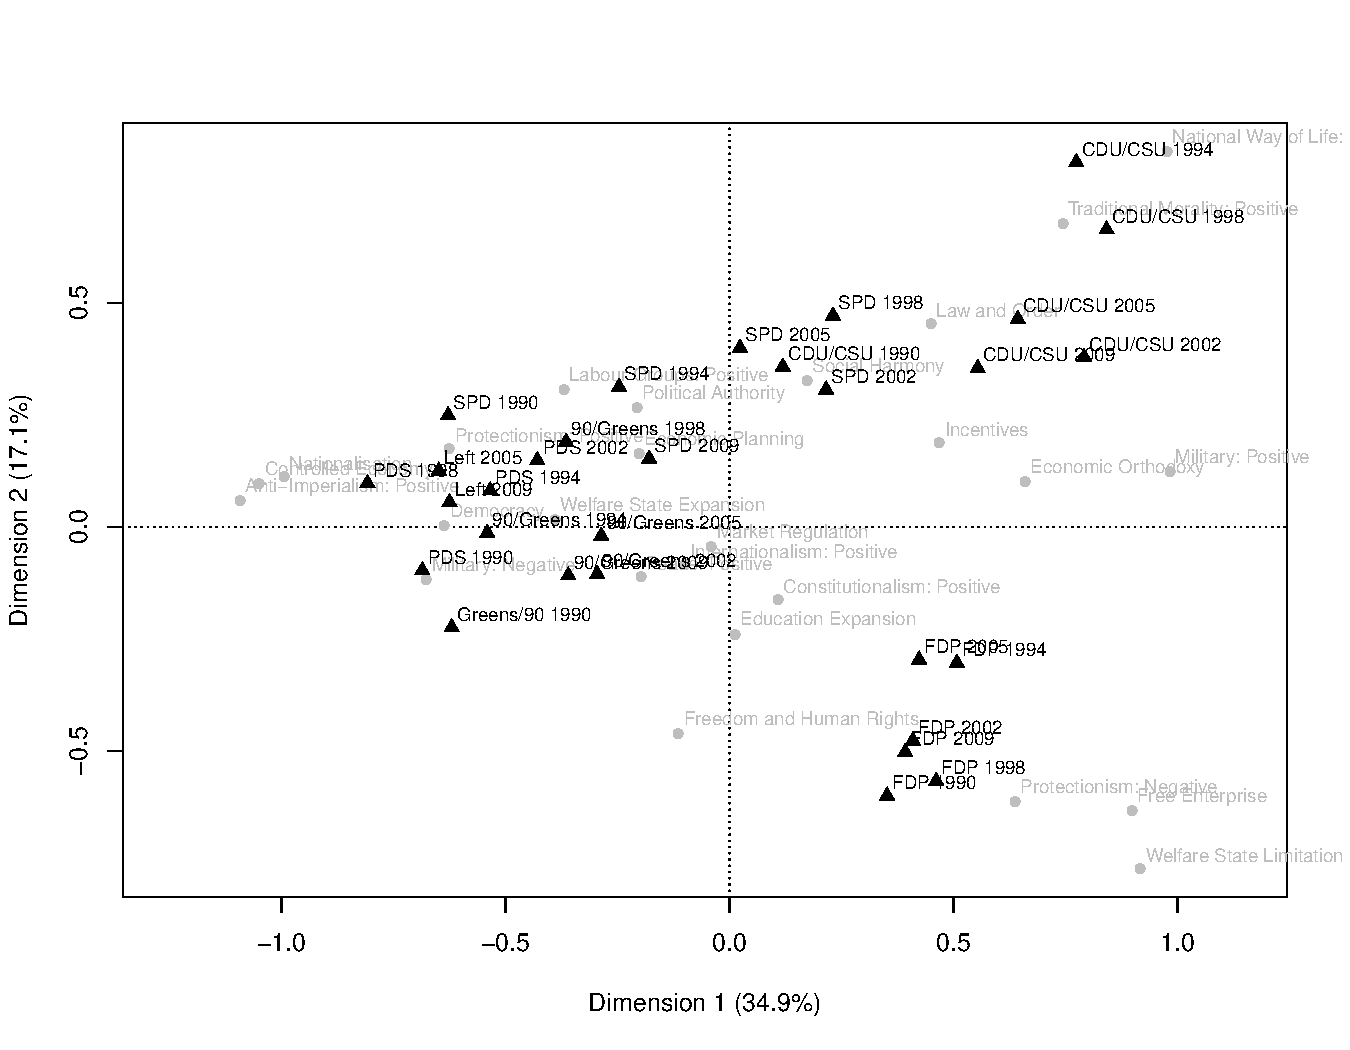
\includegraphics[scale=0.45]{pictures/grey-just-rile}}
%Post-1989 German party position from CMP-coded platforms
%
%\end{frame}

%\begin{frame}{In each other's space}
%\medskip
%\centerline{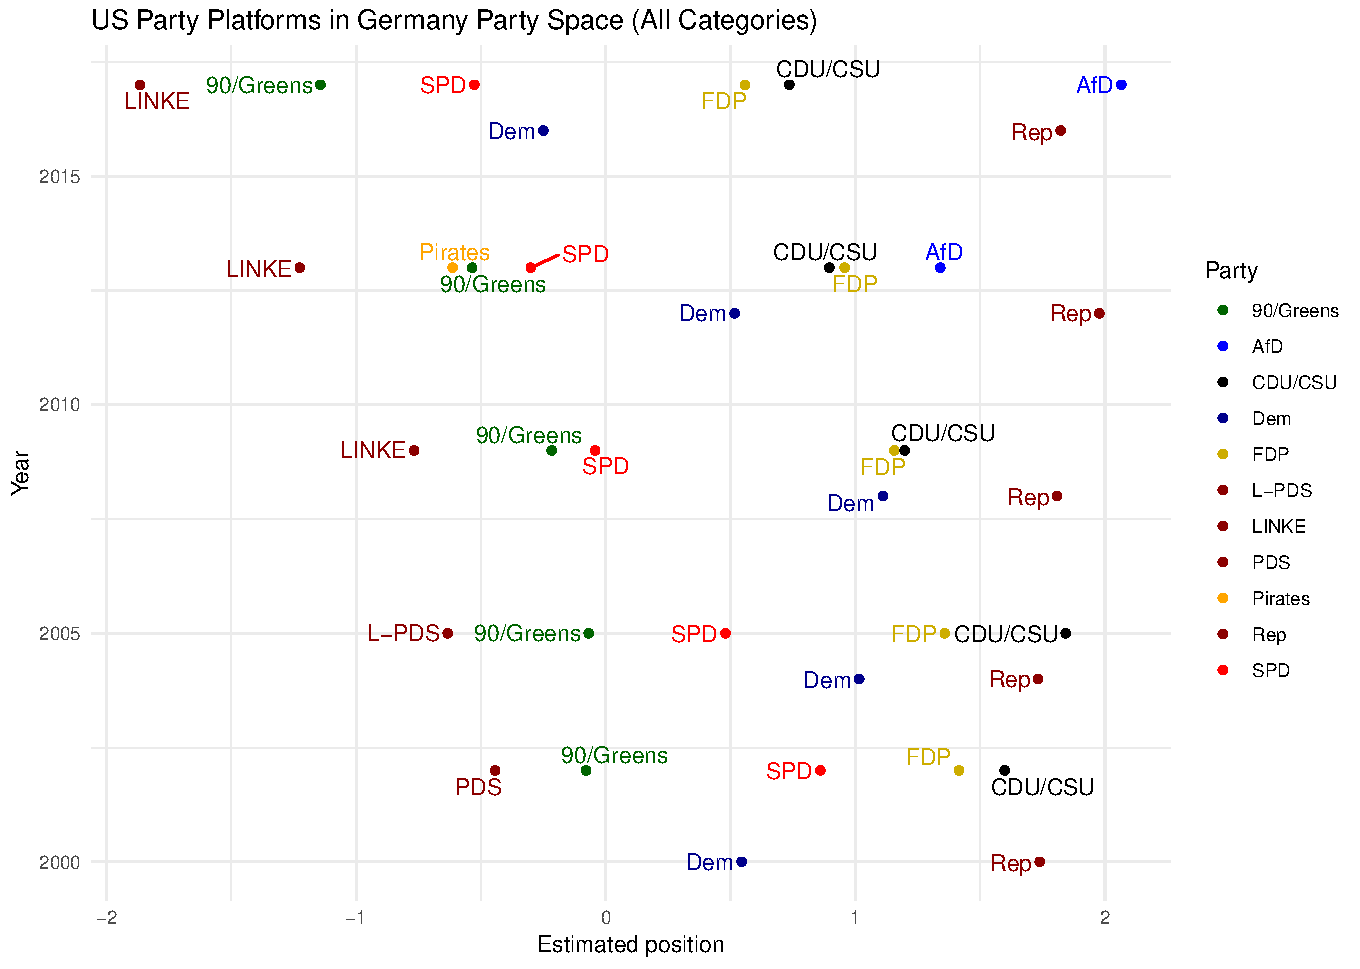
\includegraphics[scale=.35]{pictures/cmpcats_us_in_de}}
%Link: \href{https://www.nytimes.com/interactive/2019/06/26/opinion/sunday/republican-platform-far-right.html}{the pretty version at the New York Times}
%
%\end{frame}


%%%

\begin{frame}[allowframebreaks]
\frametitle{References}
\printbibliography	
\end{frame}

\end{document}